\section{Introduction}

In each kingdom of life, the diffusion of substances between the intracellular and extracellular environments is essential for cell survival.
Apart the free diffusion of small lipophilic molecules, these exchanges are mediated by transmembrane proteins of various nature, which we refer to by the term \textit{transmembrane transport proteins}, while the \textit{-omic} layer that comprises all of them is referred to as the \textit{transportome}.

The coordinated action of these proteins regulates a large number of physiological functions, such as membrane potential, nutrient absorption, waste product removal, cellular signaling, regulation of intra- and extracellular pH, and more.

While the expression of these proteins and their proper targeting are necessary prerequisites for membrane transport, they are generally not sufficient for the fulfillment of the overall function.
In fact, the establishment of \glspl{tfu}, which are capable of performing specific tasks, often requires the assembly of multiple protein subunits to form homo- or heteromultimers, or even long-range interactions among different transmembrane transport proteins.
For instance, any secondary active transporter cannot function properly in the absence of a pump that creates a chemical gradient to be dissipated.
Another example is given by the communication between \textit{STIM} calcium sensors and \textit{Orai} channels, responsible for the calcium release-activated calcium currents.

The cataloging and characterization of \glspl{tfu} can be a complex task, especially due to current limitations in proteomics research and the still low-throughput nature of the biophysical techniques for functional assays.
Currently, according to a widely accepted approximation, the individual \gls{tfu} is identified with the gene transcript of one or more subunits it consists of, assuming transcriptional levels to be directly proportional to the abundance and activity of the \glspl{tfu} they encode.
Although this approximation may have many limitations (poor correlation between transcripts and proteins, lack of functional assessment, unclear role of auxiliary subunits, \ldots), it serves as a practical approach until more precise methods for \gls{tfu} quantification and characterization become available.
% The last issue can be ameliorated under the hypothesis that transcriptional dysregulation of even one of the subunits of which it is composed may impair the functionality of the entire macromolecular complex.

According to the schema in Figure \ref{fig:BasicTree}, transport proteins can be broadly classified into two main categories: \textit{pores} and \textit{transporters}.
\begin{itemize}
    \item \textbf{Pores:} water-filled pores that allow the facilitated passage of molecules through the membrane.
    These may be additionally subdivided into \textit{ion channels} proper and \textit{aquaporins}, pores that mostly allow the passage of water.
    \item \textbf{Transporters:} proteins or protein complexes that, embedded in the membrane, allow the passage of molecules upon conformational changes.
    These may be furthermore divided into those that require ATP hydrolysis to function and those that do not, known as \textit{ATP-driven (or primary active) transporters} and \textit{\glspl{slc}}, respectively.
    A common distinction within the ATP-driven transporters is given by \textit{\gls{abc} transporters} and \textit{pumps}, where \gls{abc} transporters feature the conserved \gls{abc} domain, while pumps do not.
\end{itemize}
Overall, the phrase ``\glspl{ict}'' is now commonly used to refer to the set of all the transportome gene products that fall into one of these macro-categories.

\begin{figure}
    \centering
    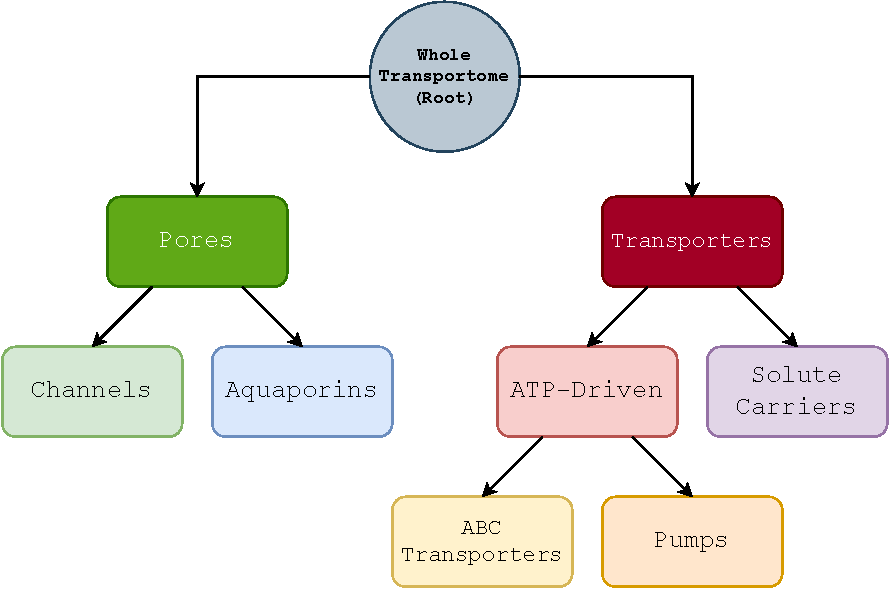
\includegraphics[width=0.65\textwidth]{resources/images/BasicTree.pdf}
    \caption{\small Tree of the principal classes of \glspl{ict}.}
    \label{fig:BasicTree}
\end{figure}

Cancer cells exhibit fundamental differences from their healthy counterparts, especially in their relationship with the extracellular environment.
Dramatic metabolic shifts are also observed in cancer.
Both of these aspects probably involve an alteration in the transportome, acting as an ``adapter''\footnote{Literally in the sense of \textit{mediator of the adaptation} towards the extracellular environment.} for cancer cells with the tumor micro-environment, while at the same time ensuring the exchange of nutrients and metabolites capable to sustain the altered metabolism.
By the above approximation, this transportome dysregulation may be reflected in the expression levels of the genes themselves, making it interesting to explore the transcriptional profile of cancer cells.

% Next two paragrahps could be even moved to Discussion 
One commonly employed approach to accomplish this task is by measuring gene expression in both healthy and diseased samples.
This is followed by \gls{dea} and enrichment analysis of the resulting gene list using ontologies---such as the \gls{go}---and hypothesis tests like hypergeometric test or Fisher's exact test.
Finally, the list of all the significantly enriched terms needs to be screened \textit{a posteriori} to search for some transportome-related terms.
The effectiveness of this process heavily relies on both the statistical power reached by the \gls{dea} and the careful curation and organization of the ontology database.

A similar---but somehow ``reversed''---approach is to generate a limited number of gene sets of interest \textit{a priori}, which meaningfully group together genes belonging to, for instance, similar \glspl{tfu}.
Then a \gls{gsea} can be performed to test them against the data and see if the function or the gene family they represent is dysregulated or not.
This second option has a few advantages:
\begin{itemize}
    \item The weighted \gls{gsea} method can take into account the magnitude of differential expression of the genes in the list (i.e., the effect size), and not their mere presence or absence.
    \item The tested gene lists may be arbitrary and not necessarily based on ontologies.
    For example, they may be manually curated, specifically crafted for a purpose (such as a list of genes involved in a specific function or pathway of interest), or generated by other methods.
    \item Given a set of features, it is possible to systematically generate all the gene sets that may be meaningfully conceived, and test them all against the data.
\end{itemize}

The present work aims at profiling the expression levels of transportome genes in the context of human cancer.
To do this, we collected information on these genes (such as their complete list, which molecule(s) they transport, their gating mechanism(s), their functional class, etc.) and used it to systematically arrange them into meaningful \glspl{tgs}.
After sorting all the protein-coding genes found in cancer cells based on their differential expression with respect to healthy cells, we ran a pre-ranked \gls{gsea} on these ordered lists to obtain enrichment scores for every \gls{tgs}.
We therefore obtained the ``dysregulation status'' of most functional facets of the transportome in $19$ different cancer tissue types.

We provide an open-source, documented, and reproducible Python package, Daedalus (\href{https://github.com/TCP-Lab/MTP-DB}{github.com/TCP-Lab/MTP-DB}) that retrieves transportome-related data from various databases and compiles it in a local \mono{.sqlite} database.
In parallel, we also provide pre-compiled database files as periodic releases.

A \mono{make}-driven and docker-containerized pipeline, named ``transportome profiler'',\\(\href{https://github.com/TCP-Lab/transportome_profiler}{github.com/TCP-Lab/transportome\_profiler}) is also available.
It takes gene expression data and the aforementioned database to generate gene sets, sorts genes based on their differential expression, and runs \gls{gsea}.
This pipeline was designed with modularity and reproducibility in mind, so that it would be easily adaptable on other datasets and databases.
